\section*{Introduction}
assefilter, detektor, data-analysesystem. 
Gassen til analyse suges ind i maskinen gennem et kapillarrr (snifferen), som kan bnes og lukkes med en mekanisk ventil (inlet valve). 
For at mindske risikoen for, at ioner fragmenterer, bliver neutraliseret eller spredt p hinanden, skal kollisionerne imelle
assefilter, detektor, data-analysesystem. 
Gassen til analyse suges ind i maskinen gennem et kapillarrr (snifferen), som kan bnes og lukkes med en mekanisk ventil (inlet valve). 
 
For at mindske risikoen for, at ioner fragmenterer, bliver neutraliseret eller spredt p hinanden, skal kollisionerne imelle \cite{RefWorks:22}

\begin{figure} 
	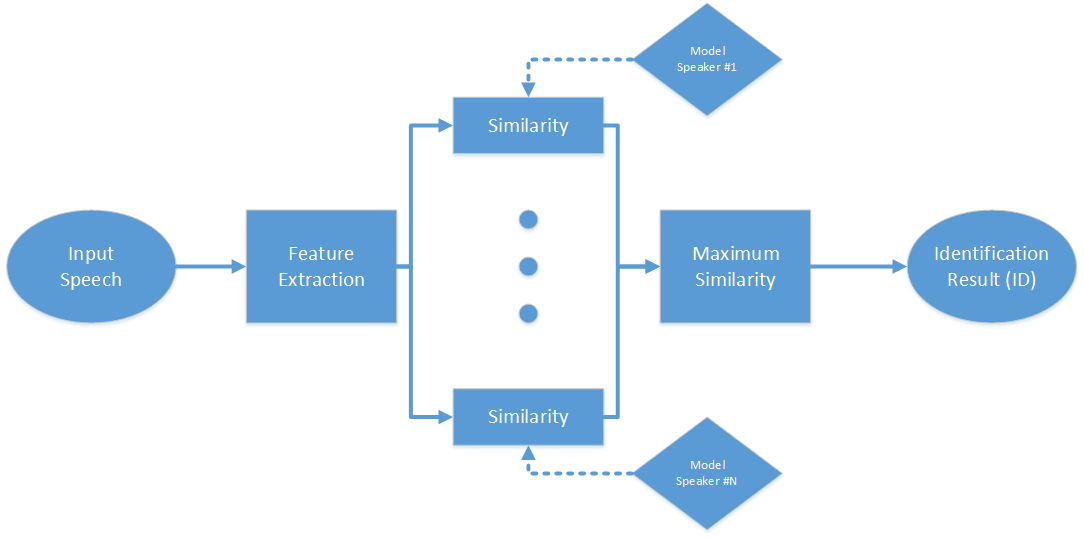
\includegraphics[width=\columnwidth]{Figures/Overview_speech_01.png}
	\caption{\textit{Show an overview of the speaker recognition}}
	\label{fig:Overview}
\end{figure}